\documentclass[12pt]{article}

\usepackage[margin=1in]{geometry}
\usepackage[T1]{fontenc}
\usepackage[utf8]{inputenc}
\usepackage{amsmath,amssymb,amsfonts,bm}
\usepackage{booktabs}
\usepackage{array}
\usepackage{caption}
\usepackage{graphicx}
\usepackage[protrusion=true,expansion=false]{microtype}
\usepackage{natbib}
\usepackage{pdflscape}
\usepackage{setspace}
\usepackage{xcolor}
\usepackage[colorlinks=true,linkcolor=blue,citecolor=blue,urlcolor=blue]{hyperref}

\graphicspath{{figures/}{outputs/}{markup_policy/}}

\newtheorem{proposition}{Proposition}
\newcommand{\E}{\mathbb{E}}
\newcommand{\RDelta}{R_{\Delta}}
\newcommand{\ytilde}{\tilde y}
\newcolumntype{C}[1]{>{\centering\arraybackslash}m{#1}}

\hypersetup{
    pdftitle={Replication of Rubbo (2023) and Oil Cost-Push Markup Shocks},
    pdfauthor={Matheus Porto Pimentel and Pedro Poliseli},
    pdfsubject={Network Phillips curves, oil markup shocks, and monetary policy},
    pdfkeywords={Rubbo, network Phillips curve, monetary policy, cost-push shocks, oil}
}

\title{Replication of Rubbo (2023) and Oil Cost-Push Markup Shocks}
\author{Matheus Porto Pimentel \and Pedro Poliseli}
\date{\today}

\begin{document}

\maketitle

\begin{abstract}
\noindent
This note documents the current replication and extension of \citet{rubbo2023networks}.
The baseline environment is a multisector New Keynesian model with input-output
linkages, sectoral price rigidities, and a divine-coincidence inflation index. We add
an oil-sector desired-markup shock, interpreted as a cost-push disturbance, and compare
simple monetary-policy responses. The current U.S. calibration shows that stabilizing
consumer-price inflation after an oil cost-push shock requires a much larger output-gap
contraction than stabilizing the divine-coincidence index. Translating the required
output gaps through the IS curve gives a direct measure of the policy-rate movement
relative to the natural rate.

\bigskip
\noindent\textbf{Keywords:} network Phillips curve; cost-push shock; oil prices;
monetary policy; divine coincidence.

\noindent\textbf{JEL Codes:} E31; E32; E52; C67.
\end{abstract}

\onehalfspacing

\section{Introduction}
\label{sec:introduction}

\citet{rubbo2023networks} revisits the New Keynesian framework in a multisector
economy with input-output linkages. The paper shows that sectoral production networks
change both the slope of Phillips curves and the inflation index that is most directly
connected to welfare. In particular, the divine-coincidence (DC) index summarizes the
inflation object that should be stabilized when productivity shocks are the relevant
disturbances.

Our extension asks a narrower policy question: how should the central bank react to an
oil-price shock when the shock is interpreted as an exogenous increase in desired
markups, rather than as a productivity disturbance? This interpretation is useful for
oil because the shock acts like a cost-push disturbance that propagates through
production chains. It also creates an inflation-output tradeoff: stabilizing CPI
inflation is possible, but it may require a large negative output gap and can move DC
inflation sharply in the opposite direction.

The note proceeds as follows. Section~\ref{sec:model} summarizes the relevant Rubbo
objects. Section~\ref{sec:costpush} introduces desired-markup shocks and the static
pass-through formulas. Section~\ref{sec:policy} describes the dynamic policy rules and
the interest-rate implementation. Section~\ref{sec:results} reports the current U.S.
calibration results. Appendix~\ref{sec:appendix-replication} keeps the replication
figures from the original exercise.

\section{Model Environment}
\label{sec:model}

The economy has $N$ industries indexed by $i,j \in \{1,\ldots,N\}$. The calibrated
primitives are the labor-share vector $\alpha$, the final-consumption weight vector
$\beta$, the input-output matrix $\Omega$, and the diagonal matrix of Calvo price
adjustment probabilities $\Delta=\mathrm{diag}(\delta_i)$. As in
\citet{rubbo2023networks}, the Domar exposure vector is
\begin{equation}
    \lambda'
    =
    \beta'(I-\Omega)^{-1}.
    \label{eq:domar}
\end{equation}

Define the rigidity-adjusted Leontief inverse and the common denominator as
\begin{equation}
    \RDelta=(I-\Omega\Delta)^{-1},
    \qquad
    d=1-\beta'\Delta\RDelta\alpha .
    \label{eq:rdeltad}
\end{equation}
Rubbo's Matlab routines then construct the sectoral Phillips-curve slope vector
\begin{equation}
    b
    =
    (\gamma+\varphi)
    \frac{\Delta\RDelta\alpha}{d},
    \qquad
    \kappa^C=\beta'b,
    \label{eq:slope}
\end{equation}
where $\gamma$ is the inverse intertemporal elasticity parameter and $\varphi$ is the
inverse Frisch elasticity parameter. The consumer-price Phillips-curve slope is
$\kappa^C$.

The sectoral Phillips curves can be written as
\begin{equation}
    \bm{\pi}_t
    =
    \rho(I-V)\E_t\bm{\pi}_{t+1}
    +
    b\,\ytilde_t
    -
    V\bm{\chi}_t,
    \label{eq:baseline-sectoral-pc}
\end{equation}
where $V$ is the sectoral network matrix, $\bm{\chi}_t$ contains productivity-driven
residual terms, and $\ytilde_t$ is the output gap. The corresponding household Euler
equation is
\begin{equation}
    \ytilde_t
    =
    \E_t\ytilde_{t+1}
    -
    \frac{1}{\gamma}
    \left(
        i_{t+1}
        -
        \E_t\pi^C_{t+1}
        -
        r^{nat}_{t+1}
    \right).
    \label{eq:is}
\end{equation}
This equation is the bridge from an output-gap path to a nominal policy-rate path.

\section{Oil Markup Cost-Push Shocks}
\label{sec:costpush}

Following Rubbo's supplement, we introduce an exogenous desired-markup shock
\begin{equation}
    \bm{\mu}^D_t \in \mathbb{R}^{N}.
    \label{eq:markup-shock}
\end{equation}
A positive entry is a cost-push shock in that sector. A targeted subsidy can be
represented as a negative markup shock, so that
\begin{equation}
    \bm{\mu}^{D,\mathrm{net}}_t
    =
    \bm{\mu}^{D,\mathrm{shock}}_t
    -
    \bm{s}_t .
    \label{eq:subsidy}
\end{equation}

The static CPI markup term computed by the Matlab module is
\begin{equation}
    v^C_t
    =
    \frac{\beta'\Delta(I-\Omega\Delta)^{-1}}
    {1-\beta'\Delta(I-\Omega\Delta)^{-1}\alpha}
    \bm{\mu}^D_t .
    \label{eq:cpi-markup}
\end{equation}
The static DC markup term is
\begin{equation}
    \pi_t^{DC}
    =
    \rho\E_t\pi_{t+1}^{DC}
    +
    (\gamma+\varphi)\ytilde_t
    +
    \lambda'\bm{\mu}^D_t .
    \label{eq:dc-markup}
\end{equation}
Thus, on impact and abstracting from expectations, the output gap that stabilizes the
DC index is
\begin{equation}
    \ytilde_t^{DC=0}
    =
    -\frac{\lambda'\bm{\mu}^D_t}{\gamma+\varphi}.
    \label{eq:dc-output-gap}
\end{equation}

The dynamic sectoral Phillips curve used in the cost-push module is
\begin{equation}
    \bm{\pi}_t
    =
    \rho(I-V)\E_t\bm{\pi}_{t+1}
    +
    b\,\ytilde_t
    +
    (I-V)\Delta(I-\Delta)^{-1}\bm{\mu}^D_t,
    \label{eq:dynamic-sectoral-pc}
\end{equation}
where the productivity term is set to zero. The oil experiment assumes an AR(1)
desired-markup process,
\begin{equation}
    \bm{\mu}^D_{t+1}
    =
    \rho_\mu \bm{\mu}^D_t.
    \label{eq:markup-ar}
\end{equation}
The Matlab code solves \eqref{eq:dynamic-sectoral-pc} backward over a finite horizon
with terminal condition $\bm{\pi}_{T+1}=0$, and reports
\begin{equation}
    \pi_t^C=\beta'\bm{\pi}_t,
    \qquad
    \pi_t^{DC}
    =
    \rho\pi_{t+1}^{DC}
    +
    (\gamma+\varphi)\ytilde_t
    +
    \lambda'\bm{\mu}^D_t.
    \label{eq:reported-inflation}
\end{equation}

\section{Policy Rules and Interest Rates}
\label{sec:policy}

The policy exercise expresses monetary policy as a path for the output gap. This is a
reduced-form implementation step: first choose the inflation object the central bank
wants to stabilize, then compute the output-gap path required to implement that
choice, and finally translate the output-gap path into an interest-rate path through
\eqref{eq:is}.

The rules currently compared are:
\begin{align}
    \ytilde_t^{0} &= 0, \label{eq:zero-gap}\\
    \ytilde_t^{DC}
    &=
    -\frac{\lambda'\bm{\mu}^D_t}{\gamma+\varphi}, \label{eq:dc-rule}\\
    \ytilde_t^{lean,CPI}
    &=
    \theta_C \ytilde_t^{CPI}, \label{eq:lean-cpi}\\
    \ytilde_t^{lean,DC}
    &=
    \theta_{DC}\ytilde_t^{DC}. \label{eq:lean-dc}
\end{align}
The CPI-stabilizing rule chooses $\ytilde_t$ so that $\beta'\bm{\pi}_t=0$ in the
backward recursion:
\begin{equation}
    \ytilde_t^{CPI}
    =
    -
    \frac{
        \rho\beta'(I-V)\bm{\pi}_{t+1}
        +
        \beta'(I-V)\Delta(I-\Delta)^{-1}\bm{\mu}^D_t
    }{
        \beta'b
    }.
    \label{eq:cpi-rule}
\end{equation}

The transparent comparison loss is quadratic:
\begin{align}
    \mathcal{L}^{CPI}
    &=
    \sum_{t=0}^{T-1}
    \rho_L^t
    \left[
        (\pi_t^C)^2+\omega_y\ytilde_t^2
    \right],
    \label{eq:loss-cpi}\\
    \mathcal{L}^{DC}
    &=
    \sum_{t=0}^{T-1}
    \rho_L^t
    \left[
        (\pi_t^{DC})^2+\omega_y\ytilde_t^2
    \right],
    \label{eq:loss-dc}\\
    \mathcal{L}^{dual}
    &=
    \sum_{t=0}^{T-1}
    \rho_L^t
    \left[
        \omega_C(\pi_t^C)^2
        +
        \omega_{DC}(\pi_t^{DC})^2
        +
        \omega_y\ytilde_t^2
    \right].
    \label{eq:loss-dual}
\end{align}
These losses are diagnostic statistics, not the full second-order welfare matrix in
\citet{rubbo2023networks}.

Rearranging the IS curve gives the policy-rate movement relative to the natural rate:
\begin{equation}
    i_{t+1}-r^{nat}_{t+1}
    =
    \E_t\pi^C_{t+1}
    +
    \gamma
    \left(
        \E_t\ytilde_{t+1}-\ytilde_t
    \right).
    \label{eq:rate-gap}
\end{equation}
The code uses the simulated future paths as model-consistent expectations, with
terminal values set to zero:
\begin{equation}
    \widehat i_{t+1}
    \equiv
    i_{t+1}-r^{nat}_{t+1}
    =
    \pi^C_{t+1}
    +
    \gamma
    \left(
        \ytilde_{t+1}-\ytilde_t
    \right).
    \label{eq:rate-implemented}
\end{equation}
Because the exercise is a desired-markup shock rather than a productivity shock, the
reported $\widehat i_{t+1}$ is the policy-rate response above the natural-rate path.

\section{Results}
\label{sec:results}

The current baseline is a 10 percent desired-markup shock in the oil sector with
$\rho_\mu=0.80$, using the U.S. 2012 calibration from the replication files.
Table~\ref{tab:oil_cpi_original} reproduces the oil productivity-shock benchmark,
while Tables~\ref{tab:oil_markup_cpi} and~\ref{tab:markup_dc_response} report the new
cost-push markup calculations.

The distinction between the productivity-shock benchmark and the markup-shock exercise
is important. In the original oil experiment, the disturbance changes the productive
capacity of the oil sector and therefore enters the Phillips curves through the
productivity residuals. In the extension, the disturbance raises desired markups and is
therefore closer to a cost-push shock: firms would like to charge a higher relative
price even without a change in physical productivity. This is the relevant experiment
for asking how monetary policy should react to an adverse oil-price movement that looks
like a supply-driven increase in marginal costs.

\begin{table}[htbp]
    \centering
    \caption{Consumer inflation after a $10\%$ negative oil-sector productivity shock}
    \label{tab:oil_cpi_original}
    \begin{tabular}{lccc}
        \toprule
        & \multicolumn{3}{c}{Full model} \\
        \cmidrule(lr){2-4}
        & $\delta =$ actual
        & $\delta \equiv \delta_{\mathrm{mean}},\ \delta_{\mathrm{oil}}=1$
        & $\delta \equiv \delta_{\mathrm{mean}}$ \\
        \midrule
        Sticky wages   & 0.22 & 0.07 & $-0.00$ \\
        Flexible wages & 0.18 & 0.01 & $-0.06$ \\
        \bottomrule
    \end{tabular}
    \begin{flushleft}
        \footnotesize
        \textit{Notes:} Values are percentage points. This table is the original
        oil-shock benchmark from the Rubbo replication code.
    \end{flushleft}
\end{table}

Table~\ref{tab:oil_cpi_original} is a useful benchmark because it shows how much of
the original oil result comes from the joint role of price rigidity, wage rigidity, and
input-output propagation. With actual sectoral price-adjustment probabilities, a
10 percent negative oil-sector productivity shock raises consumer inflation by
0.22 percentage points under sticky wages and by 0.18 percentage points under flexible
wages. The sticky-wage case is larger because wage rigidity prevents part of the
adjustment from occurring through wages, so more of the disturbance appears in goods
prices. When all sectors are assigned the mean price flexibility but the oil sector is
kept fully flexible, the response falls to 0.07 and 0.01 percentage points. When all
sectors receive the mean value of $\delta$, the CPI effect is essentially zero under
sticky wages and slightly negative under flexible wages. The table therefore says that
oil is not important only because it is an expenditure item; it matters because oil is
located in the production network and because its price rigidity differs from the
average sector.

\begin{table}[htbp]
    \centering
    \caption{CPI response to a $10\%$ oil-sector markup shock}
    \label{tab:oil_markup_cpi}
    \begin{tabular}{lccc}
        \toprule
        & $\delta =$ actual
        & $\delta \equiv \delta_{\mathrm{mean}},\ \delta_{\mathrm{oil}}=1$
        & $\delta \equiv \delta_{\mathrm{mean}}$ \\
        \midrule
        CPI response & 0.242 & 0.084 & 0.016 \\
        \bottomrule
    \end{tabular}
    \begin{flushleft}
        \footnotesize
        \textit{Notes:} Values are percentage points. The underlying Matlab outputs
        are $0.0024183$, $0.00083976$, and $0.00015828$, respectively.
    \end{flushleft}
\end{table}

Table~\ref{tab:oil_markup_cpi} repeats the oil experiment but changes the nature of
the shock. The markup shock produces a 0.242 percentage-point CPI response under the
actual calibration, slightly larger than the sticky-wage productivity benchmark in
Table~\ref{tab:oil_cpi_original}. This happens because the desired-markup shock enters
directly as a cost-push term: it is not mediated by productivity and therefore creates
inflationary pressure even when output is held fixed. The alternative $\delta$
experiments again show that sectoral price rigidity is central. Setting all sectors to
the mean $\delta$ while making oil fully flexible lowers the CPI response to
0.084 percentage points, and setting all sectors to the mean $\delta$ lowers it further
to 0.016 percentage points. The sharp decline indicates that the calibrated
heterogeneity in adjustment probabilities is doing substantial work in the static
pass-through calculation.

\begin{table}[htbp]
    \centering
    \caption{CPI, divine-coincidence inflation, and output-gap response}
    \label{tab:markup_dc_response}
    \begin{tabular}{lccc}
        \toprule
        & CPI markup
        & DC markup
        & Output gap stabilizing DC \\
        \midrule
        Response & 0.002418 & 0.006851 & $-0.002284$ \\
        \bottomrule
    \end{tabular}
    \begin{flushleft}
        \footnotesize
        \textit{Notes:} Values are decimal units. In percentage points, the
        responses are $0.242$, $0.685$, and $-0.228$, respectively.
    \end{flushleft}
\end{table}

Table~\ref{tab:markup_dc_response} explains why the monetary-policy problem is not
well summarized by CPI alone. The CPI markup term is 0.002418 in decimals, or
0.242 percentage points. The DC markup term is 0.006851, or 0.685 percentage points,
almost three times as large. This gap arises because the DC index weights sectors by
their network relevance for the divine-coincidence condition, while CPI weights sectors
by final-consumption exposure. Oil has a larger role as an upstream input than as a
direct final-consumption item, so the network-based inflation pressure is larger than
the consumer-price pressure. The output gap that stabilizes DC inflation on impact is
$-0.002284$, or $-0.228$ percentage points. This number is the first measure of the
real activity cost of stabilization: keeping the network-relevant inflation object
stable requires a contraction, but a relatively modest one compared with the
CPI-stabilizing rule shown below.

Figure~\ref{fig:markup-dynamic-irf} shows the dynamic inflation responses to the oil
markup shock. CPI inflation rises on impact and gradually decays as the AR(1) markup
shock dies out. The DC response is much larger on impact and also more persistent in
levels, reflecting the fact that the shock travels through the input-output network
before reaching final prices. This is the dynamic counterpart of
Table~\ref{tab:markup_dc_response}: CPI is the object consumers see directly, but DC is
the object that internalizes the upstream pressure created by oil as an intermediate
input. The figure also shows the illustrative subsidy experiment. Offsetting part of
the oil-sector markup reduces the CPI response at every horizon, but it does not change
the qualitative propagation mechanism: the shock still fades gradually because the
underlying markup process is persistent.

\begin{figure}[htbp]
    \centering
    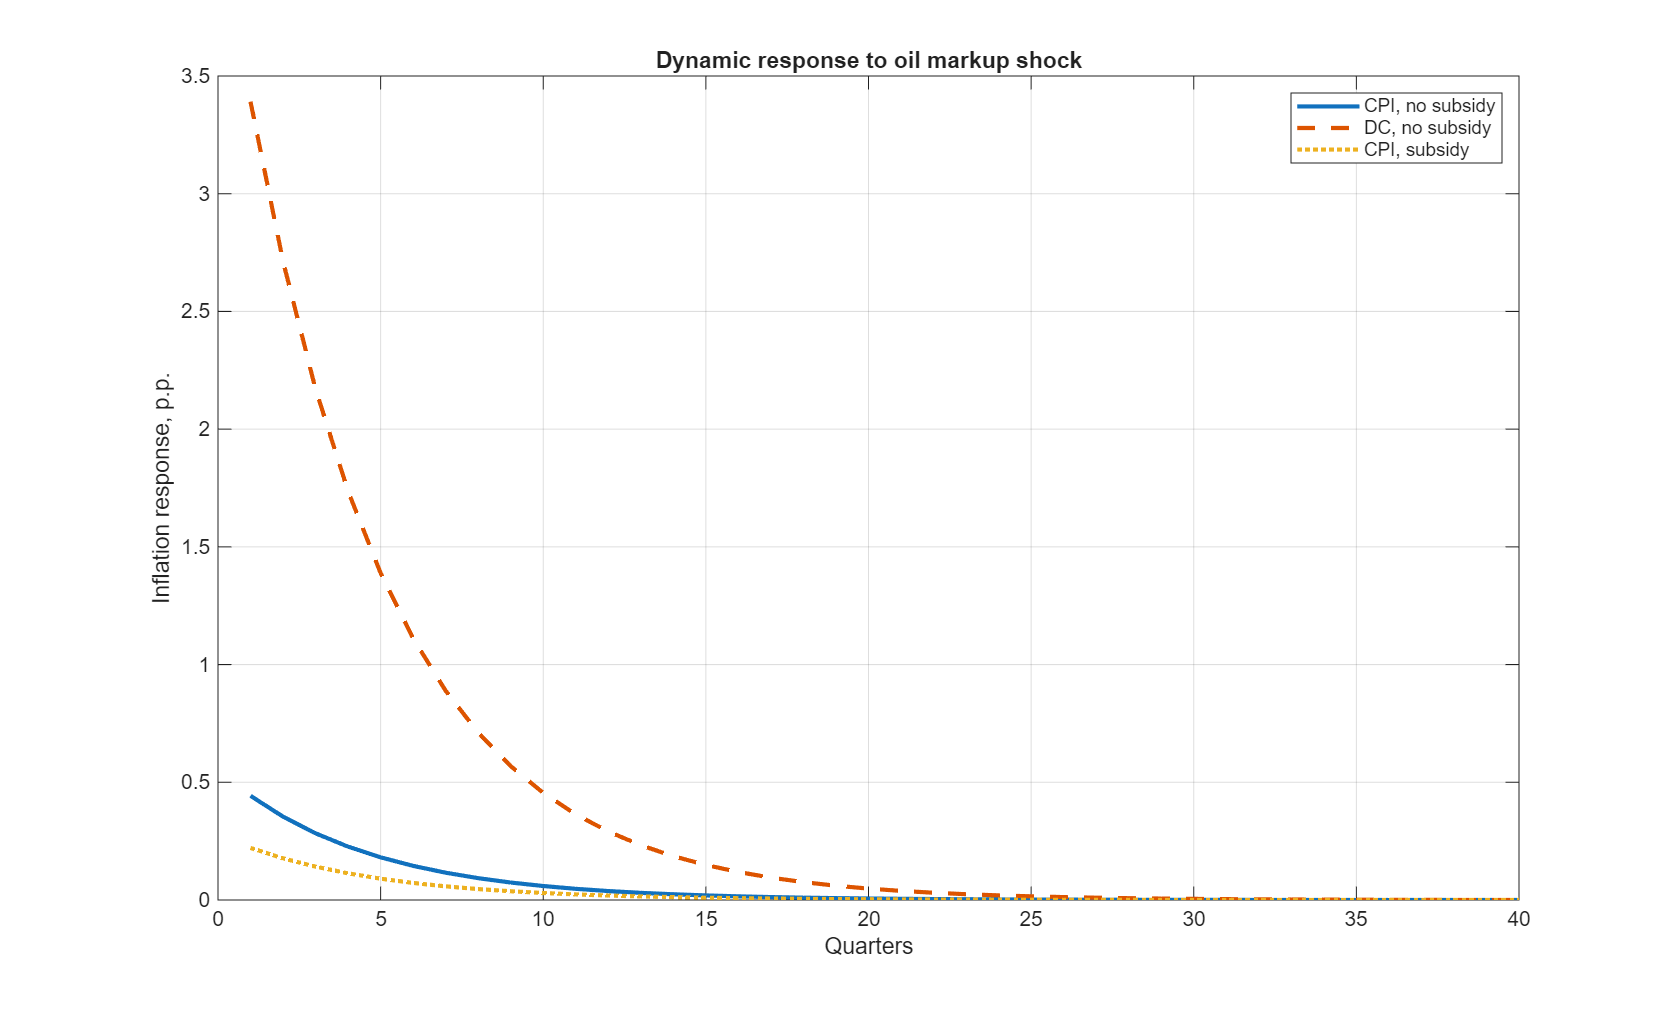
\includegraphics[width=0.92\textwidth]{oil_markup_dynamic_irf.png}
    \caption{Dynamic inflation response to an oil-sector markup shock}
    \label{fig:markup-dynamic-irf}
\end{figure}

Figure~\ref{fig:network-pressure} summarizes the network-pressure object generated by
the sectoral Phillips-curve markup term. The no-subsidy line is the chain-wide pressure
created by the oil cost-push shock. Its impact value is much larger than the CPI
response because this object aggregates sectoral pressure before final-consumption
weights compress it. The subsidy line shows how a targeted offset reduces propagated
pressure along the production chain, not merely the direct oil-sector price. This is
important for policy design: a sectoral fiscal instrument can dampen the source of the
network shock, while monetary policy can only trade off inflation stabilization against
the output gap.

\begin{figure}[htbp]
    \centering
    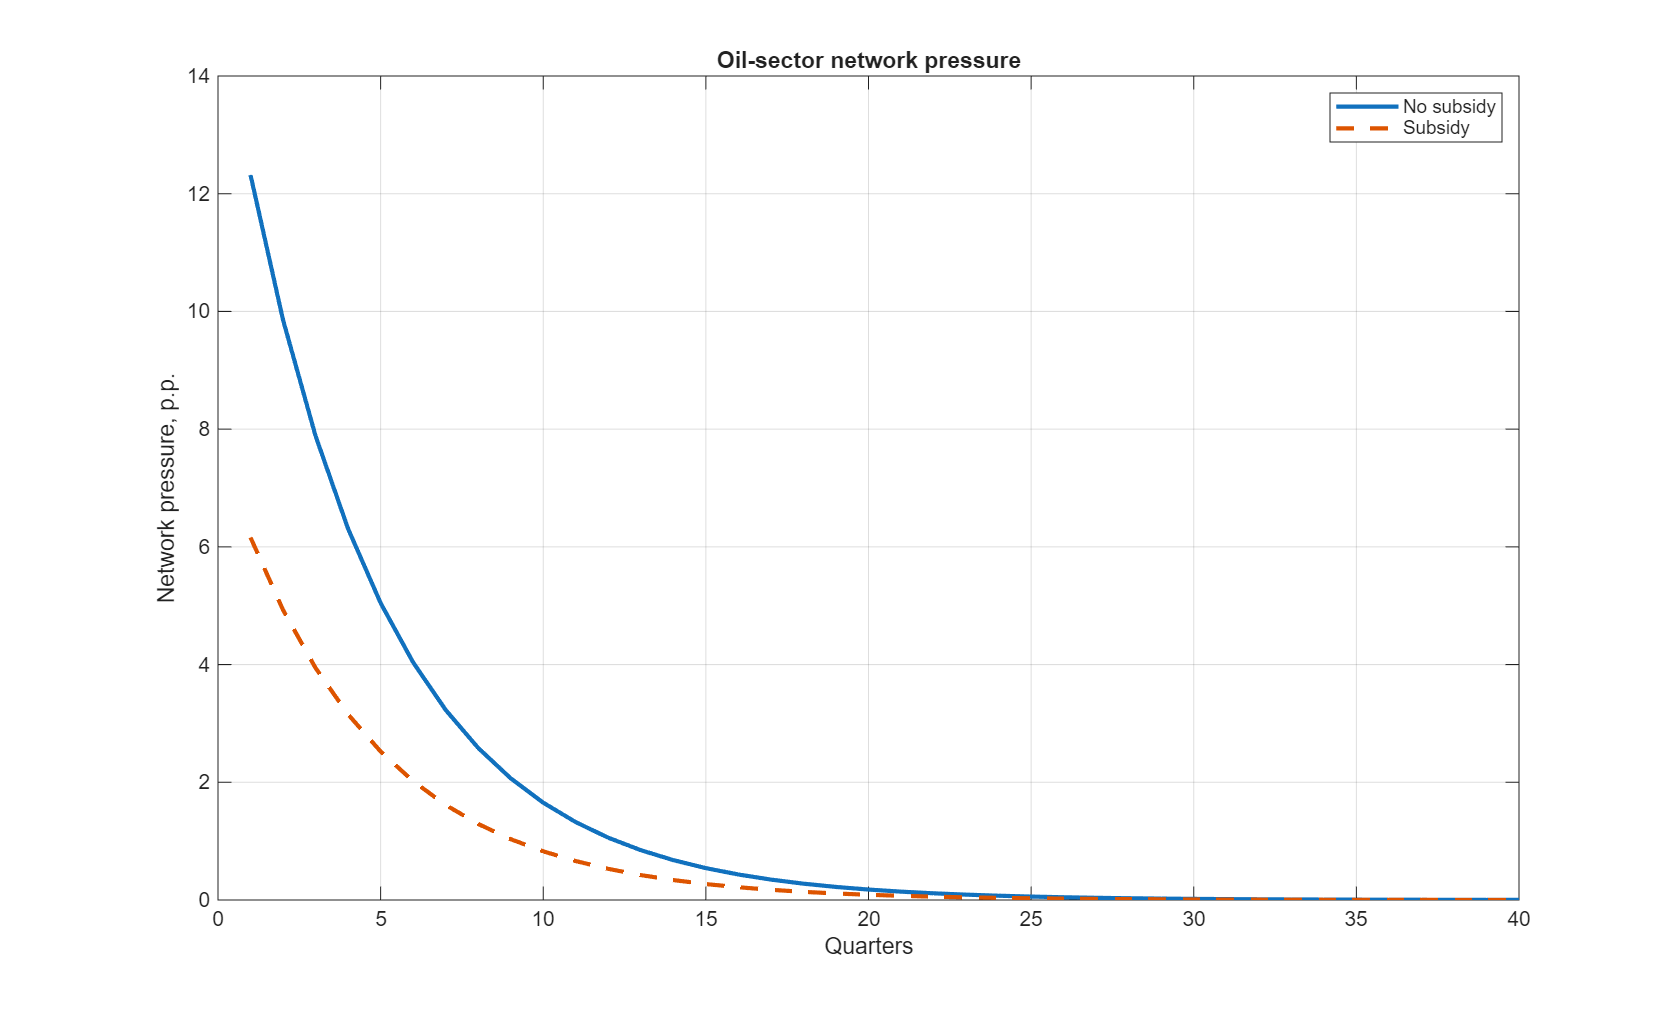
\includegraphics[width=0.92\textwidth]{oil_markup_network_pressure.png}
    \caption{Network pressure from the oil-sector markup shock}
    \label{fig:network-pressure}
\end{figure}

\subsection{Monetary-Policy Comparison}
\label{subsec:policy-results}

Figures~\ref{fig:policy-cpi}--\ref{fig:policy-loss} compare the five policy rules. The
rules should be read as different answers to the same central-bank question. The
zero-gap rule asks what inflation does if the central bank does not move real activity
in response to the oil markup shock. The CPI-stabilizing rule asks how contractionary
policy must be to keep consumer-price inflation at zero. The DC-stabilizing rule asks
how much policy must move output to stabilize the network-relevant inflation index. The
two lean-against rules are partial responses, halfway between accommodation and exact
stabilization.

Figure~\ref{fig:policy-cpi} focuses on consumer-price inflation. By construction, the
CPI-stabilizing rule keeps the CPI response at zero. The zero-gap rule produces the
largest CPI response, because monetary policy does not create any offsetting demand
contraction. The DC-stabilizing rule still lowers CPI inflation relative to the
zero-gap benchmark, but it does not eliminate it. This is the main policy tradeoff:
stabilizing the inflation index that is most closely connected to the production
network allows some temporary movement in the consumer price index.

\begin{figure}[htbp]
    \centering
    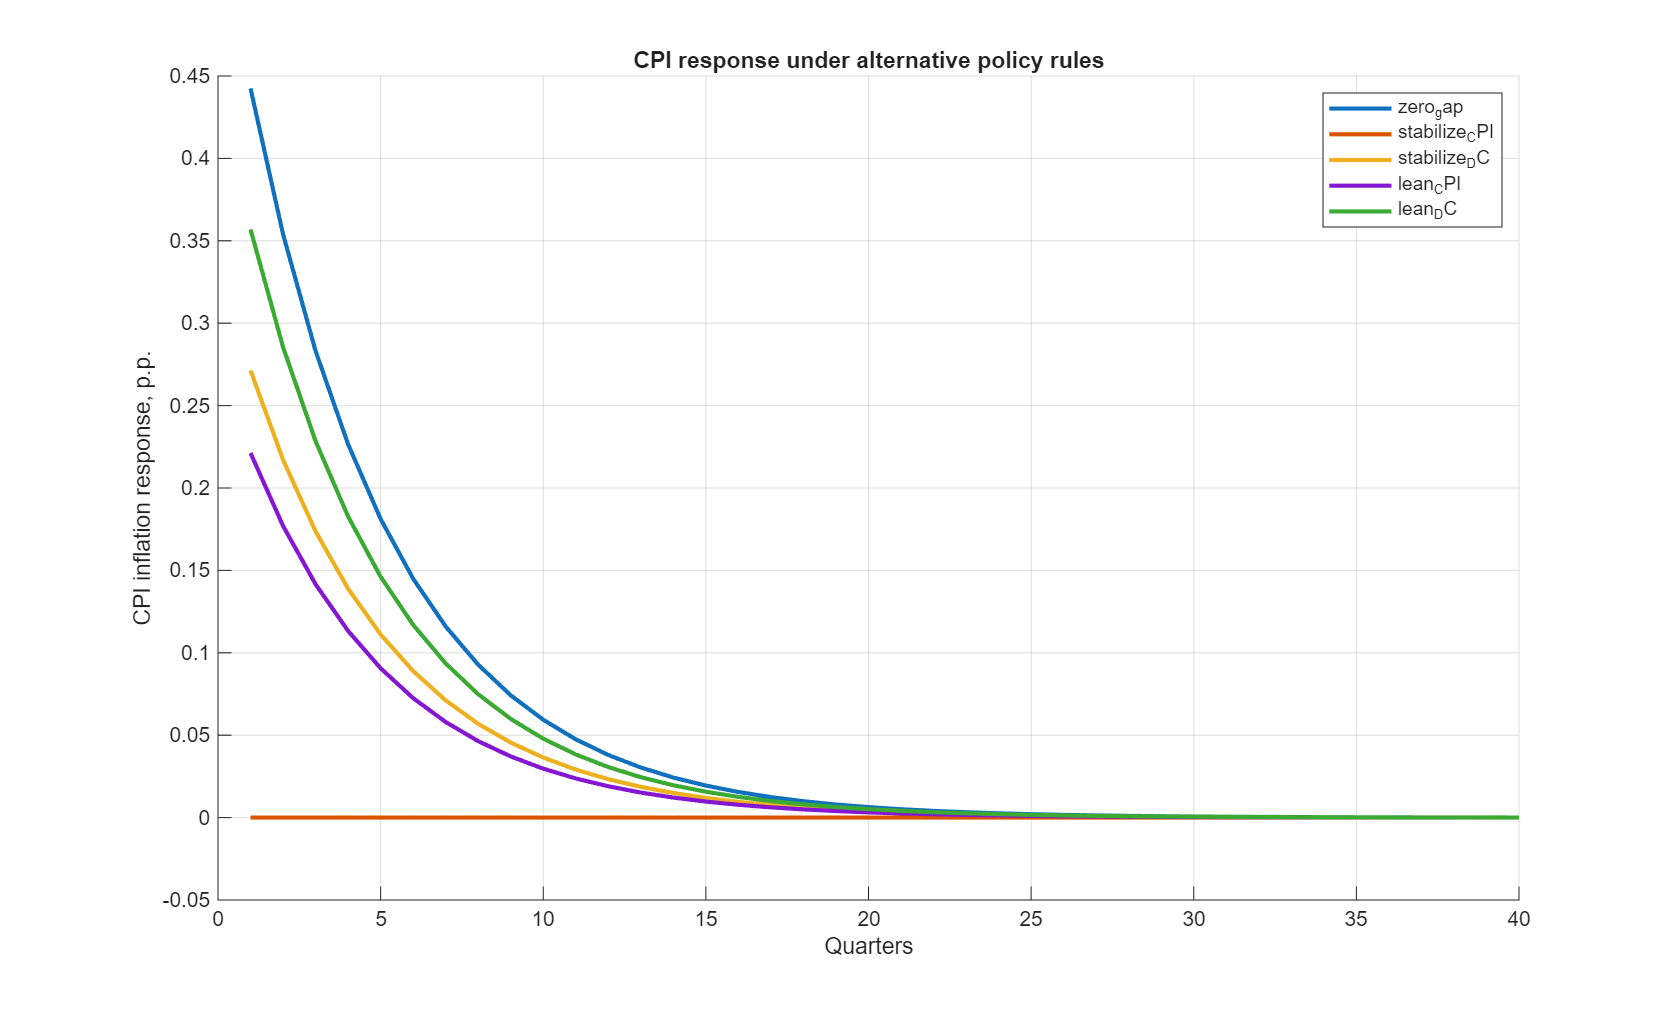
\includegraphics[width=0.92\textwidth]{policy_CPI_responses.png}
    \caption{CPI response under alternative monetary-policy rules}
    \label{fig:policy-cpi}
\end{figure}

Figure~\ref{fig:policy-dc} reverses the ranking. The DC-stabilizing rule sets the
divine-coincidence response to zero, while the CPI-stabilizing rule generates a large
negative DC response. The reason is mechanical but economically revealing: to eliminate
CPI inflation after an oil cost-push shock, policy must engineer a sizeable negative
output gap. That contraction more than offsets the DC markup term, so the DC index
undershoots. In other words, strict CPI stabilization may look successful from the
perspective of headline inflation while creating an excessive contraction relative to
the network-based stabilization criterion.

\begin{figure}[htbp]
    \centering
    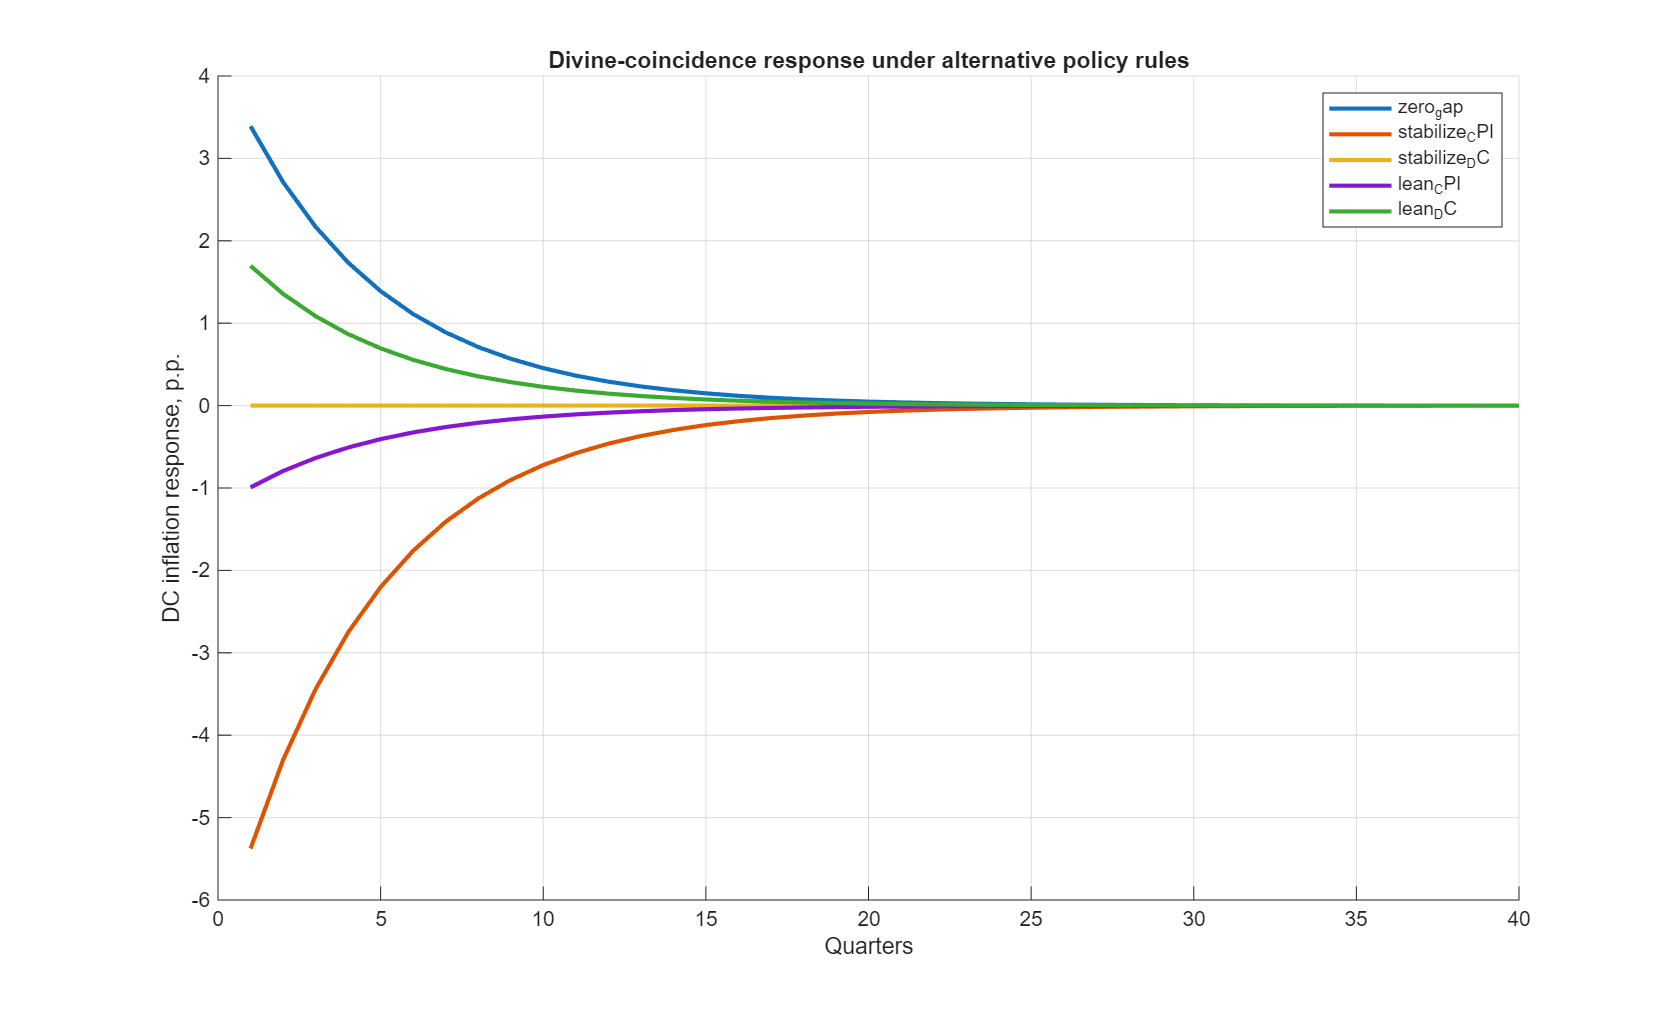
\includegraphics[width=0.92\textwidth]{policy_DC_responses.png}
    \caption{Divine-coincidence inflation response under alternative monetary-policy rules}
    \label{fig:policy-dc}
\end{figure}

Figure~\ref{fig:policy-gap} makes the real-side cost explicit. The zero-gap rule has
no output response by construction. The CPI-stabilizing rule requires the deepest
contraction, with an impact output gap close to $-0.59$ percentage points. The
DC-stabilizing rule requires a smaller contraction, around $-0.228$ percentage points
on impact. The partial rules sit between these extremes. This figure is especially
useful for interpreting the policy problem: the central bank can always reduce
inflation by contracting demand, but the relevant question is whether the additional
inflation stabilization is worth the additional output loss.

\begin{figure}[htbp]
    \centering
    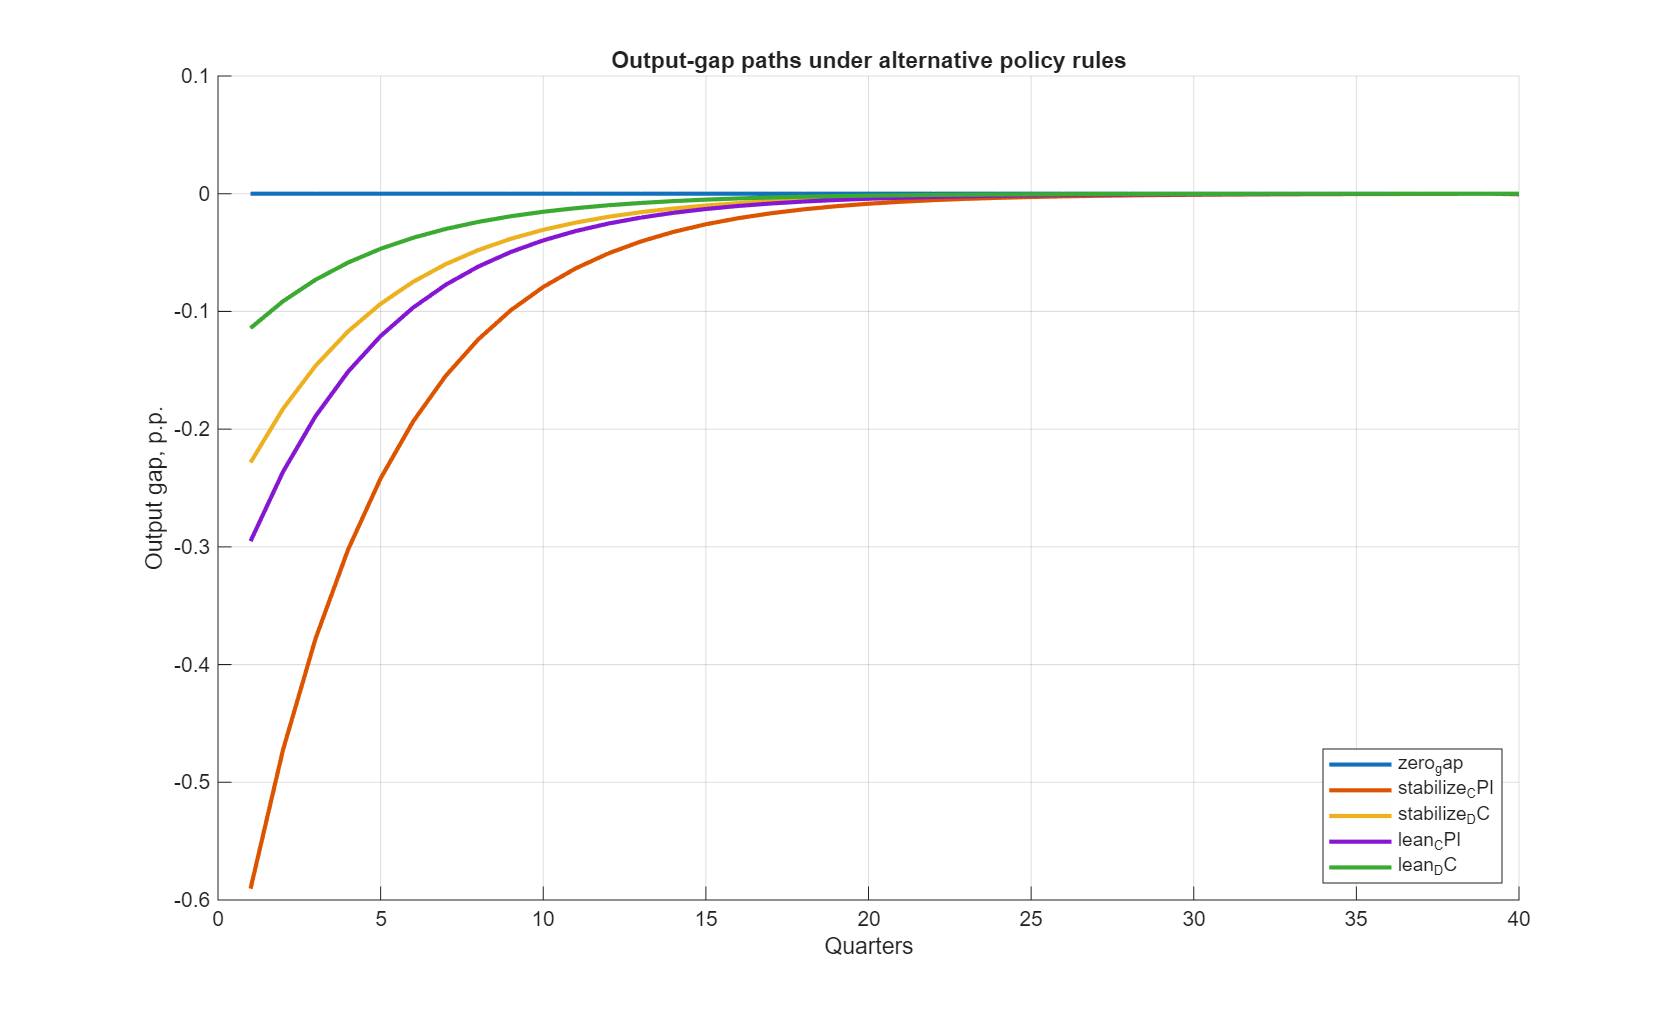
\includegraphics[width=0.92\textwidth]{policy_output_gap_paths.png}
    \caption{Output-gap paths under alternative monetary-policy rules}
    \label{fig:policy-gap}
\end{figure}

Figure~\ref{fig:policy-loss} summarizes these tradeoffs in the diagnostic quadratic
losses. A CPI-only loss rewards the CPI-stabilizing rule for eliminating headline
inflation, but still penalizes the output contraction required to do so. A DC loss
penalizes the CPI-stabilizing rule heavily because that rule creates a large DC
undershooting. Under the dual criterion, which cares about both CPI and DC inflation
as well as the output gap, the DC-stabilizing rule performs best in this calibration.
The result should not be interpreted as a full welfare ranking yet, since the loss here
is intentionally transparent and not Rubbo's full welfare matrix. It is nevertheless a
clear diagnostic: a central bank that reacts only to CPI may over-tighten after an oil
cost-push shock.

\begin{figure}[htbp]
    \centering
    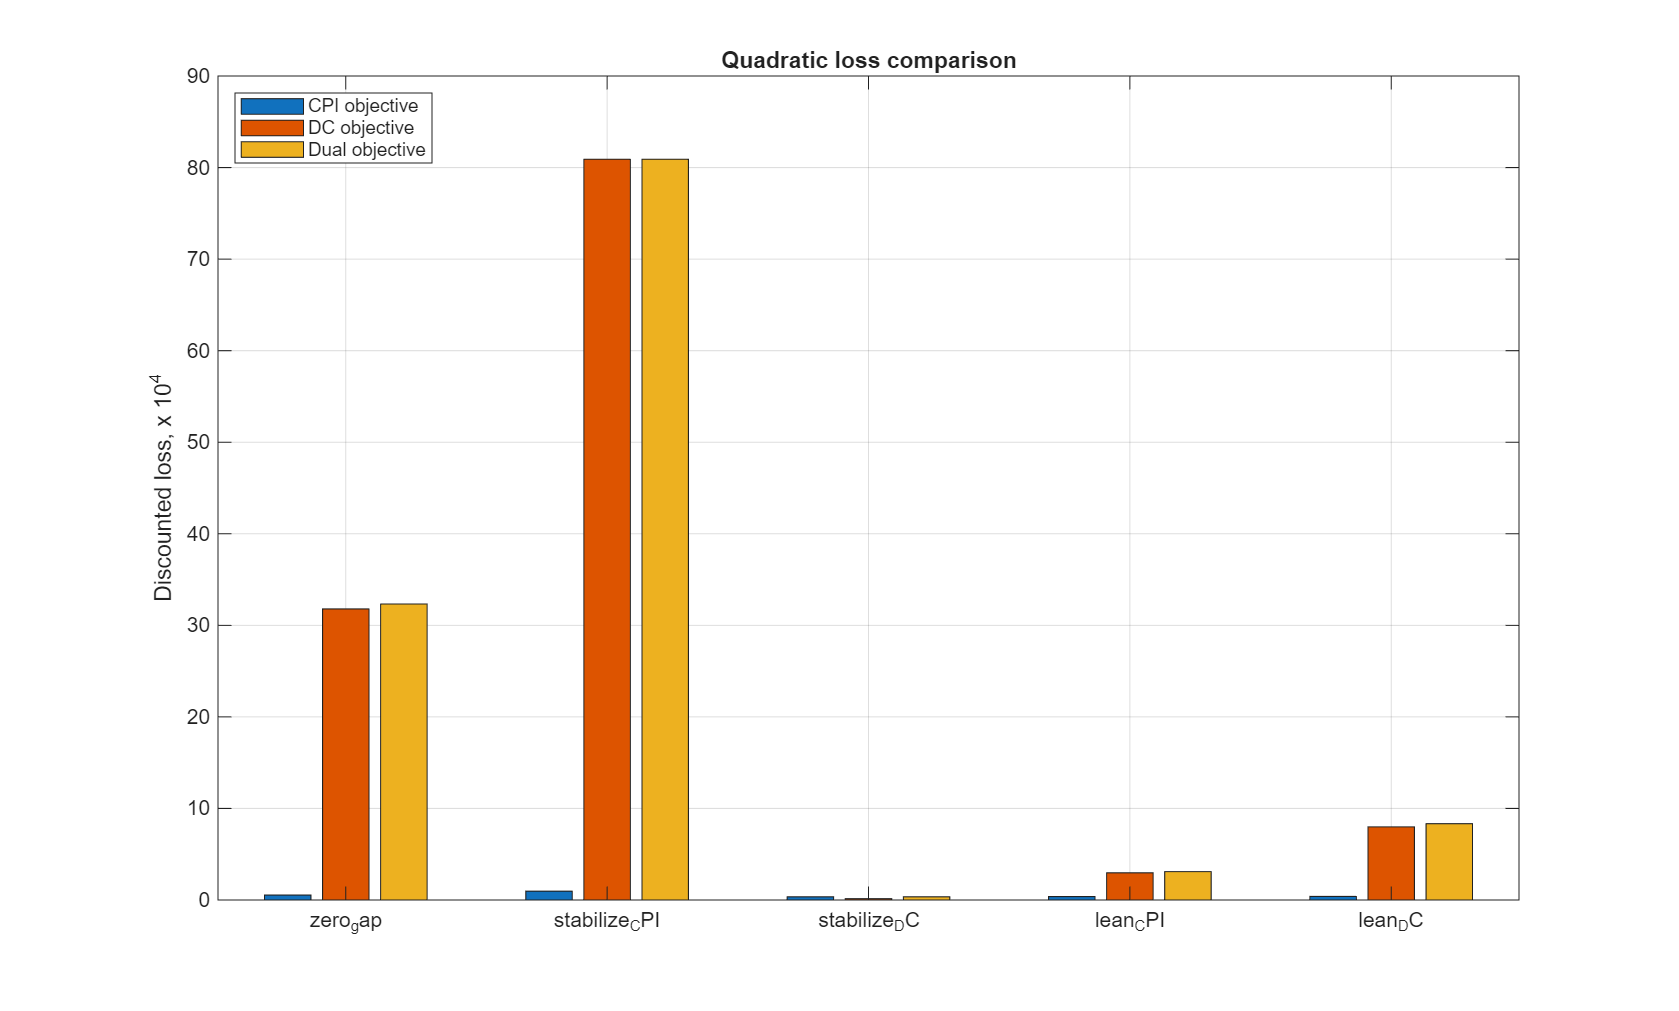
\includegraphics[width=0.92\textwidth]{policy_loss_comparison.png}
    \caption{Quadratic loss comparison under alternative monetary-policy rules}
    \label{fig:policy-loss}
\end{figure}

Table~\ref{tab:summary_policy_rules} reports the same comparison numerically. The
zero-gap rule has no output cost, but it allows a peak CPI response of
0.442 percentage points and a peak DC response of 3.391 percentage points. Its total
loss is therefore dominated by DC inflation. The strict CPI rule eliminates CPI
inflation, but it requires the largest output movement, 0.590 percentage points in
absolute value, and generates the largest DC deviation, 5.377 percentage points. This
is why its DC and total losses are the highest in the table. The strict DC rule sets
the peak DC response to zero, leaves a peak CPI response of 0.271 percentage points,
and requires a smaller output gap of 0.228 percentage points. It therefore minimizes
the DC loss and the total loss in the current diagnostic criterion. The two lean-against
rules show the value of partial accommodation: leaning against CPI lowers CPI inflation
relative to zero-gap policy but still keeps DC deviations limited, while leaning
against DC uses the smallest nonzero output response but leaves more inflation
volatility.

\begin{table}[htbp]
    \centering
    \caption{Summary statistics under alternative monetary-policy rules}
    \label{tab:summary_policy_rules}
    \resizebox{\textwidth}{!}{%
        \begin{tabular}{lcccccc}
            \toprule
            Policy rule
            & Peak $|\pi^{CPI}|$
            & Peak $|\pi^{DC}|$
            & Max $|\ytilde|$
            & Loss CPI $\times 10^{4}$
            & Loss DC $\times 10^{4}$
            & Total loss $\times 10^{4}$ \\
            \midrule
            Zero output gap      & 0.442 & 3.391 & 0.000 & 0.541 & 31.792 & 32.334 \\
            Stabilize CPI        & 0.000 & 5.377 & 0.590 & 0.964 & 80.907 & 80.907 \\
            Stabilize DC         & 0.271 & 0.000 & 0.228 & 0.348 & 0.144  & 0.348  \\
            Lean against CPI     & 0.221 & 0.993 & 0.295 & 0.376 & 2.968  & 3.103  \\
            Lean against DC      & 0.357 & 1.696 & 0.114 & 0.388 & 7.984  & 8.336  \\
            \bottomrule
        \end{tabular}%
    }
    \begin{flushleft}
        \footnotesize
        \textit{Notes:} Inflation and output-gap responses are percentage points.
        Losses are reported in units of $10^{-4}$. Numerical zeros correspond to
        values close to machine precision.
    \end{flushleft}
\end{table}

Table~\ref{tab:rate_policy_rules} converts the output-gap rules into policy-rate
movements relative to the natural rate using \eqref{eq:rate-implemented}. These
responses should be interpreted carefully. They are not policy-rate levels and they are
not deviations from the pre-shock nominal rate. They are the nominal rate movements
above the natural-rate path needed to implement each output-gap rule through the IS
curve. Because the experiment is a pure markup shock, the productivity component of the
natural rate is unchanged in the current implementation.

The zero-gap rule requires an impact rate increase of 0.354 quarterly percentage
points, or 1.416 annualized percentage points. This is the rate movement that prevents
the output gap from moving despite higher expected CPI inflation. The strict
CPI-stabilizing rule requires a smaller rate-gap movement, 0.118 quarterly percentage
points or 0.472 annualized percentage points, because the rule deliberately allows a
large contemporaneous negative output gap. The interest-rate formula contains
$\gamma(\ytilde_{t+1}-\ytilde_t)$; when policy creates a sharp negative output gap on
impact that subsequently closes, this expected recovery partly substitutes for a larger
rate increase. The DC-stabilizing rule requires 0.263 quarterly percentage points, or
1.051 annualized percentage points. It is therefore more contractionary in interest-rate
space than strict CPI stabilization, but much less contractionary in output-gap space.
This distinction is central: the severity of a policy rule cannot be read from the
interest-rate response alone; it must be read jointly with the output-gap path.

The two partial rules make the same point. Leaning against CPI requires an annualized
rate response of 0.944 percentage points and a maximum output gap of
0.295 percentage points. Leaning against DC requires a larger annualized rate response,
1.233 percentage points, but a smaller output-gap movement of 0.114 percentage points.
The ranking differs because the IS curve maps rates into the change in the output gap,
not only into the level of the output gap. For the current calibration, the preferred
rule under the diagnostic loss is not the rule with the smallest rate response; it is
the rule that best balances CPI inflation, DC inflation, and output stabilization.

\begin{table}[htbp]
    \centering
    \caption{Interest-rate responses under alternative monetary-policy rules}
    \label{tab:rate_policy_rules}
    \resizebox{\textwidth}{!}{%
        \begin{tabular}{lcccc}
            \toprule
            Policy rule
            & Impact, q. p.p.
            & Peak $|q|$, p.p.
            & Impact, ann. p.p.
            & Peak $|ann.|$, p.p. \\
            \midrule
            Zero output gap  & 0.354 & 0.354 & 1.416 & 1.416 \\
            Stabilize CPI    & 0.118 & 0.118 & 0.472 & 0.472 \\
            Stabilize DC     & 0.263 & 0.263 & 1.051 & 1.051 \\
            Lean against CPI & 0.236 & 0.236 & 0.944 & 0.944 \\
            Lean against DC  & 0.308 & 0.308 & 1.233 & 1.233 \\
            \bottomrule
        \end{tabular}%
    }
    \begin{flushleft}
        \footnotesize
        \textit{Notes:} Quarterly responses are percentage points. Annualized
        responses multiply the quarterly rate by four.
    \end{flushleft}
\end{table}

\section{Conclusion}
\label{sec:conclusion}

The current exercise suggests that the answer to the policy question depends on which
inflation index the central bank treats as the relevant target after an oil cost-push
shock. If it insists on stabilizing CPI exactly, the model requires a large output-gap
contraction and generates a severe movement in DC inflation. If it stabilizes the DC
index, the output contraction is smaller and the diagnostic loss is lower, while CPI
inflation is allowed to move temporarily. The next step is to connect this reduced-form
policy comparison to Rubbo's full welfare matrix and then rebuild the primitives
$\alpha$, $\beta$, and $\Omega$ with Brazilian input-output data.

\clearpage
\singlespacing
\bibliographystyle{plainnat}
\bibliography{references}

\clearpage
\onehalfspacing
\appendix

\section{Replication Figures from Rubbo's Baseline}
\label{sec:appendix-replication}

This appendix keeps the figures produced by the baseline replication routines. They
are useful checks on the calibrated objects before adding the oil markup-shock layer.

\begin{figure}[htbp]
    \centering
    \includegraphics[width=0.86\textwidth]{Figure_1.png}
    \caption{Welfare losses under alternative policy rules in the baseline replication}
    \label{fig:rubbo-baseline-losses}
\end{figure}

\begin{figure}[htbp]
    \centering
    \includegraphics[width=0.86\textwidth]{Figure_2.png}
    \caption{CPI and divine-coincidence Phillips-curve slopes over time}
    \label{fig:rubbo-pc-slopes}
\end{figure}

\begin{figure}[htbp]
    \centering
    \includegraphics[width=0.86\textwidth]{Figure_3.png}
    \caption{Consumption shares and pass-through changes in the baseline replication}
    \label{fig:rubbo-pass-through}
\end{figure}

\begin{figure}[htbp]
    \centering
    \includegraphics[width=0.86\textwidth]{Figure_4.png}
    \caption{Wage Phillips-curve slope over time in the baseline replication}
    \label{fig:rubbo-wage-pc}
\end{figure}

\end{document}
